\section{Experiments} \label{sec:experiments}





Our algorithm is implemented in Python using \textsc{PyTorch} for autodifferentiation. Our comparisons to Iterative Closest Point and its derivative works, Deep Closest Point \cite{wang2019deep}, and Instant3dit \cite{barda2025instant3dit} use official or publicly available implementations \cite{Zhou2018}. We render our results using \textsc{Blender}, and provide more implementation details in the Supplementary Materials.

% bvh
As is theoretically expected, our main computational bottleneck is the calculation of point-to-mesh distances involved in the proximity and IPC losses $\mathcal{L}_p$ and $\mathcal{L}_{IPC}$.
Our tailor-made BVH reduces the computational cost of this step, allowing us to produce results for relatively large meshes within reasonable times (see Supplementary).


\begin{wrapfigure}[10]{r}{0.50\linewidth}
    \vspace{-4mm}
    \centering
    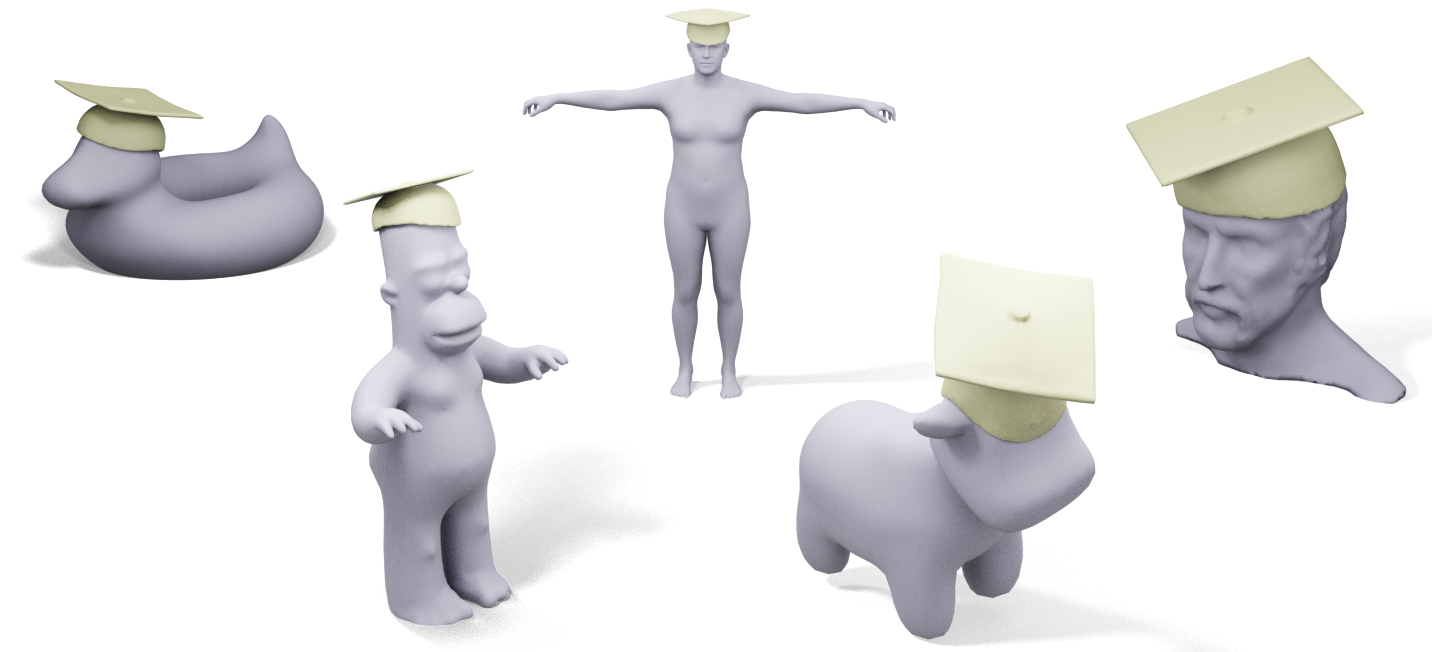
\includegraphics[width=\linewidth]{figures/same_accesory_different_base/same_accesory_different_base.png}
    \caption{}
    % \caption{Our method fits the same accessory on different base meshes, adapting to differences in scale, head shape, and body proportions to place the asset in a semantically correct position.}
    \label{fig:same_accesory_different_base}
\end{wrapfigure}





\begin{figure*}[t]
    \vspace{3mm}
    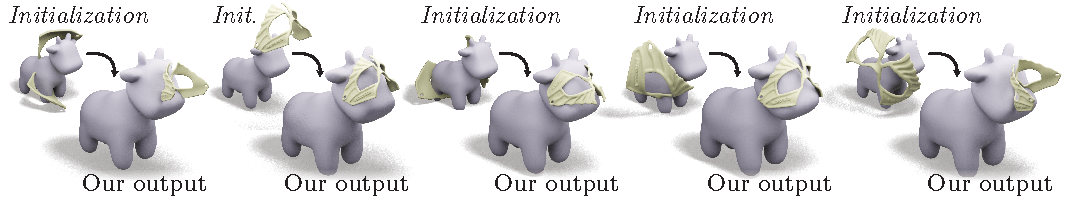
\includegraphics[width=\textwidth]{figures/placeholders/initialization.pdf}   
    \caption{Our method is moderately robust to different initialization configurations, although it can fail to converge to the desired output in very adversarial cases (leftmost and rightmost). In \autoref{sec:initialization}, we introduce a VLM initialization strategy that avoids these cases.}
    \label{fig:initialization}
    \vspace{-4mm}
\end{figure*}


% highlight robustness
A particularly relevant set of parameters are the material elastic properties $\lambda$ and $\mu$, which can be derived from the material's Young's modulus and Poisson's ratio \cite{sifakis2012fem}.
These quantities are tabulated for well-known materials; however, we make the process more intuitive for an artist by assigning the values from text inputs using an LLM. We explore both the VLM assignment and the effect of these parameters in \autoref{fig:materials}, in which the object is allowed to deform more or less depending on the specified material.

As expected, our algorithm's output is most sensitive to the selected target region on the base mesh $\highlightedfaces\subset \basefaces$.
In \autoref{fig:highlight-region}, we show how this input can allow artists to select different semantically meaningful assembly configurations between the two objects in ambiguous cases.
A similar example is given in \autoref{fig:four_fingers}, where different highlight regions specify the finger wearing a ring.



To obtain a tight, non-intersecting fit between the base and the accessory, our algorithm relies on a VLM-driven initialization and four successive optimizations, the input and output of each we show in \autoref{fig:main_method}. In \autoref{fig:steps-ablation}, we show the importance of each of these steps: skipping the VLM initialization results in a non-semantic fit (a backwards hat), while skipping any of the intermediate steps results in outputs with significantly worse physical and geometric fit. As expected, skipping Step 4 results in a strictly rigid fit, while enabling Step 4 allows the object to deform.

Critically, in Step 2 of our algorithm (\autoref{sec:step2}), we sample trajectories to find a close, non-intersecting configuration. We exemplify this in \autoref{fig:trajectory_method}; as shown in \autoref{fig:steps-ablation}, skipping this causes the barrier term in Step 3 to greatly displace the shape away from the base mesh.



\section{Comparisons} \label{sec:comparisons}
% ICP and deep closest point
\subsection{Qualitative Evaluation}
Inspired by the digital artists' workflows, we consider the specific question of how to align two pre-existing shapes in a semantically meaningful, non-intersecting, tight way.
While the lack of prior work dedicated to this particular problem makes direct comparisons difficult, we justify the need for our method by showing the failure of existing general-purpose algorithms when applied to this task.

For example, by finding an alignment between two 3D objects, our method can be seen as a special kind of \emph{registration} algorithm. However, unlike standard registration algorithms, we do not rely on the existence of a rigid geometric match between the two objects: as shown in \autoref{fig:materials}, the accessory may need to deform significantly for it to even be a partial match of the base mesh.

\begin{figure}[t]
    \vspace{3mm}
    \centering
    
    \begin{subfigure}[t]{0.49\linewidth}
        \centering
        \begin{minipage}[t][0.8cm][t]{\linewidth}
            \centering\textbf{(a) Ring Placement}
        \end{minipage}
        \phantomsubcaption\label{fig:four_fingers}
        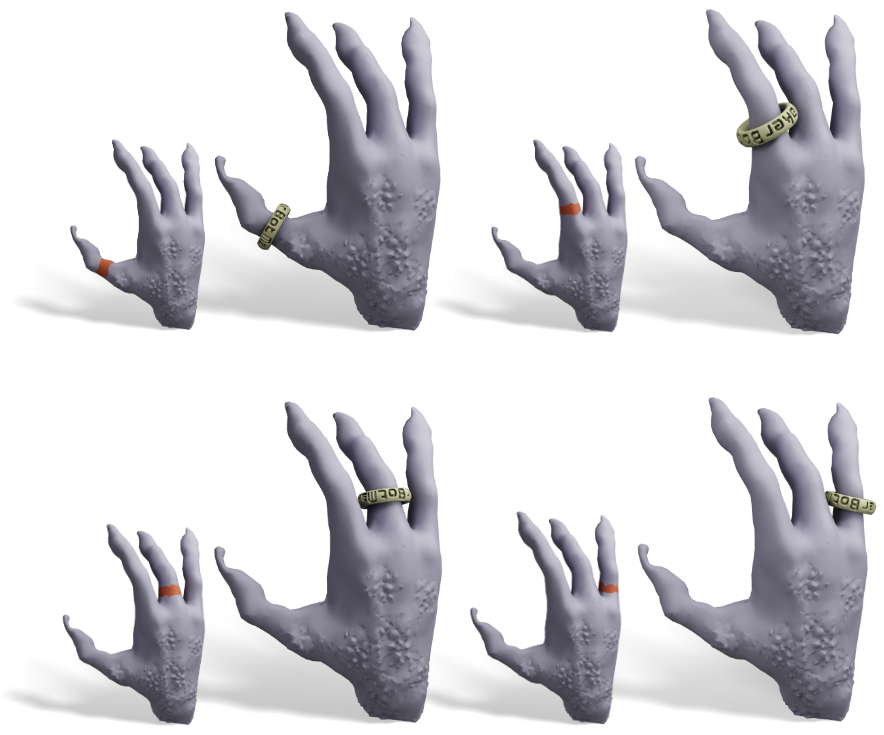
\includegraphics[width=\linewidth]{figures/region_control/four_fingers.png}
    \end{subfigure}
    \hfill
    \begin{subfigure}[t]{0.49\linewidth}
        \centering
        \begin{minipage}[t][0.8cm][t]{\linewidth}
            \centering\textbf{(b) Region Sensitivity}
        \end{minipage}
        \phantomsubcaption\label{fig:highlight-region}
        
\includegraphics[width=\linewidth]{figures/region_control/highlight-region-2-2.pdf}
    \end{subfigure}

    \vspace{3mm}
    \caption{
    \textbf{Region-controlled composition.}
    \textbf{(a)} Given four distinct user-selected target regions, \ourmethod{} places a ring precisely on each selected region, demonstrating explicit user control over the fitting process.
    \textbf{(b)} Because the method adheres strictly to the selected region, asset placement is sensitive to the region definition; for example, glasses sit naturally on the ears only if a small portion of the ear region is included in the selection.
    }
    \label{fig:region_control}
\end{figure}

More importantly, general shape registration algorithms, which are often used with point cloud inputs, will cause significant intersections between the base mesh and the object.
We show examples of this phenomenon in \autoref{fig:comparison}, where we compare our method to variants of classical registration methods \cite{besl1992method}\footnote{\label{fn:alignment_baseline}Classical registration methods are highly sensitive to bad initialization, so we use their variants that are known to be more robust. More details can be found in the Supplementary Materials.}.
Additionally, non-neural methods like those based on the Iterative Closest Point algorithm will not account for the semantic fit between the two objects; \eg, fitting the glasses backwards on the face.
We also experimented with public implementations of data-driven methods like Deep Closest Point \cite{wang2019dcp}; however, we found that these struggle greatly with most standard shapes outside of their training data, when restricted to the highlighted target region.

By modifying a shape using diffusion guidance, a highlighted region, and an optional text prompt, our work may seem similar to existing text-guided generative mesh-editing works.
Unlike these, however, our work preserves both the object and base meshes as well as any information stored in them.
Taking Instant3dit \cite{barda2025instant3dit} as a representative example, we show the difference between ours and this class of methods in \autoref{fig:instant3dit_comparison}.
Instant3dit produces a generative edit that merges the geometry of both objects and discards the animation rig of the base mesh and the parametrization of the accessory.
By contrast, our method places a world of possibilities in the hands of the artist by preserving all these, enabling common downstream tasks like animation, physical simulation, and texture painting.

\begin{figure*}[t]   
    \vspace{3mm}
    \centering
    % \vspace{-0.5cm}
    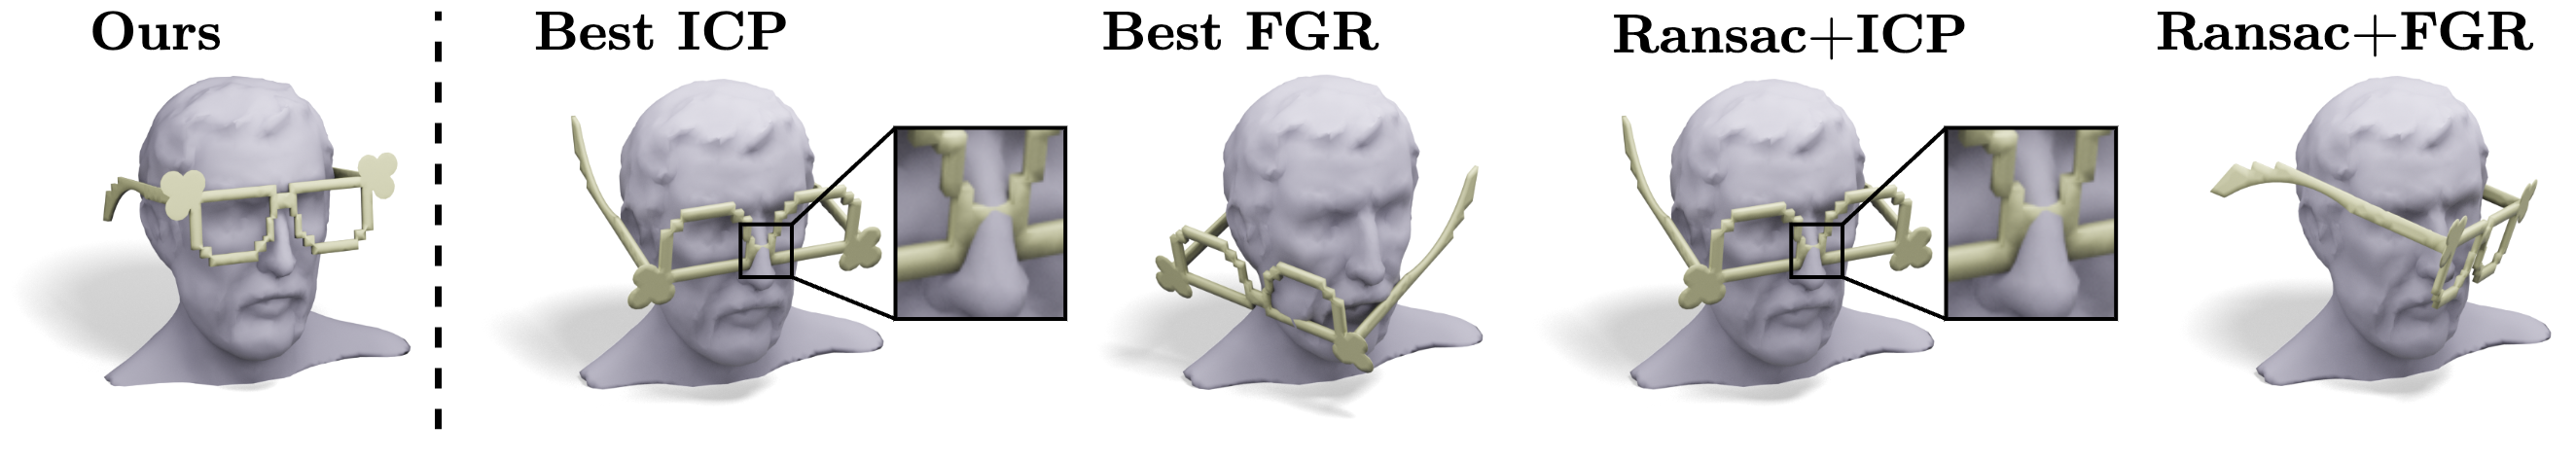
\includegraphics[width=\textwidth]{figures/comparison/comparison.png}
        \captionof{figure}{Unlike ours (left), classical registration algorithms like ICP contain no semantic guidance: therefore, they will produce unrealistic configurations; e.g., glasses that sit on the eyes upside down. These algorithms are also not designed to avoid intersections; therefore, they will produce many of them (see blowups). See supplementary materials for details of these methods.}
    %\vspace{-2cm}
    \label{fig:comparison}
\end{figure*}%



\subsection{Quantitative Evaluation.}
We quantitatively evaluate our method along two complementary dimensions: semantic alignment quality and geometric validity. We also show a user study of semantic alignment in the Supplementary Materials.\\

In \autoref{tab:quant_all}, we  compare our method against multiple alignment baselines, including Instant3Dit~\cite{barda2025instant3dit}, Best ICP/FGR, and RANSAC-based variants~\ref{fn:alignment_baseline}.  
We measure semantic quality using VQA~\cite{lin2024evaluating} and two CLIP-based metrics~\cite{radford2021learning,wang2023exploring} on image renderings of ten examples. We post examples of these renderings in the Supplementary Materials.
Across these metrics, our full method achieves the strongest or near-strongest performance (for CLIP-IQA scores, the margin is $0.006\text{--}0.009$).
Alignment-based methods also frequently produce mesh intersections, an undesirable artifact for most graphics workflows. 
In \autoref{tab:penetration} we report total intersecting faces and maximum penetration depth for each for these methods, demonstrating that while all baseline methods exhibit substantial intersections, our method produces intersection-free compositions. 







\section{Applications} \label{sec:applications}
% teaser
% same accessory, different base mesh
% gallery
% different regions, same meshes
% beanie
Since our method is designed to fit directly into artists' workflows, we prioritize providing them with the highest degree of control over the fit, automating only the tedious rigid and deformable fitting procedure.
With our method, artists may specify every creative detail: from the input meshes and their properties, which are preserved (see \autoref{fig:instant3dit_comparison}), to the accessory's material parameters (see \autoref{fig:materials}) and the specific region of the fit (see \autoref{fig:four_fingers}).

\begin{table}[t]
\vspace{4mm}
\centering
\small
\setlength{\tabcolsep}{6pt}
\renewcommand{\arraystretch}{1.2}
\setlength{\aboverulesep}{0pt}
\setlength{\belowrulesep}{0pt}

\resizebox{\columnwidth}{!}{%
\begin{tabular}{lcccccc}
\toprule
\multicolumn{7}{l}{\textbf{Alignment Baselines}}\\
\rowcolor{headercolor}
Metric & \shortstack{Instant3Dit} & \shortstack{Best ICP} & \shortstack{Best FGR} & \shortstack{RANSAC+ICP} & \shortstack{RANSAC+FGR} & \shortstack{Ours} \\
\midrule
\rowcolor{zebra}
CLIP ($\uparrow$)     & 0.311 & 0.341 & 0.333 & 0.331 & 0.321 & \textbf{0.356} \\
CLIP-IQA ($\uparrow$) & 0.559 & 0.586 & 0.609 & 0.608 & \textbf{0.610} & 0.604 \\
\rowcolor{zebra}
VQA ($\uparrow$)      & 65.62 & 73.71 & 73.97 & 73.72 & 73.68 & \textbf{74.49} \\
\midrule
\\[4pt] 
\midrule
\multicolumn{7}{l}{\textbf{Ablation Study}}\\
\rowcolor{headercolor}
Metric & \shortstack{Init} & \shortstack{Step 1} & \shortstack{Step 2} & \shortstack{Step 3} & \shortstack{Step 4} & \shortstack{Ours} \\
\midrule
\rowcolor{zebra}
CLIP ($\uparrow$)     & 0.338 & 0.351 & 0.346 & 0.347 & 0.354 & \textbf{0.356} \\
CLIP-IQA ($\uparrow$) & 0.594 & 0.605 & 0.609 & 0.595 & \textbf{0.613} & 0.604 \\
\rowcolor{zebra}
VQA ($\uparrow$)      & 74.197 & 73.967 & 73.776 & 74.049 & 73.985 & \textbf{74.49} \\
\bottomrule
\end{tabular}%
}
\vspace{4mm}
\caption{Quantitative evaluation using CLIP, CLIP-IQA, and VQA scores. Top: comparison against alignment baselines. Bottom: ablation study of our multi-step pipeline. Scores are averaged over per-example best renderings (best of 4); higher is better.}
\vspace{-2mm}
\label{tab:quant_all}
\end{table}

We exemplify our algorithm's applicability through several prototypical examples. As shown in \autoref{fig:gallery}, our method can find tight, non-intersecting configurations between a diverse range of meshes, even when these contain complex geometries, concavities, and topologies.
In \autoref{fig:teaser}, successive pre-existing shapes are added to an existing model to create a superhero character.
Conversely, in \autoref{fig:same_accesory_different_base}, the same accessory is automatically placed on a wide range of characters, demonstrating how our method can adapt to different scales, head shapes, and body proportions.



\begin{table}[t]
\vspace{4mm}
\centering
\small
\setlength{\tabcolsep}{3pt}
\renewcommand{\arraystretch}{1.15}

\begin{tabularx}{\linewidth}{>{\raggedright\arraybackslash}X c c c c c}
\toprule
{\textbf{Ablation Study}}\\
\rowcolor{headercolor}
Metric &
Best ICP &
Best FGR &
RANSAC+ICP &
RANSAC+FGR &
Ours \\
\midrule
\rowcolor{zebra}
Intersecting faces ($\downarrow$)
& 628 & 660 & 544 & 434 & \textbf{0} \\
Max penetration ($\downarrow$)
& 0.0197 & 0.0237 & 0.0243 & 0.0237 & \textbf{0} \\
\bottomrule
\end{tabularx}
\vspace{4mm}
\caption{Penetration statistics averaged over ten experiments. We report the total number of intersecting faces and the maximum penetration depth. Our method produces intersection-free compositions (all zeros).}
\vspace{-3mm}
\label{tab:penetration}
\end{table}